\documentclass[svgnames,tikz]{standalone}
\usetikzlibrary{positioning,arrows.meta,calc, backgrounds}
\usepackage{lmodern}


\tikzset{
   class/.style={draw, fill=LightYellow},
   template/.style={label={[mTemplateNodeStyle]north east:#1}},
   realization/.style={-Latex[open]},
%%
   mTemplateNodeStyle/.style={fill=white,draw,dashed,font={\tt\small}, inner sep=2pt, anchor=center}
}


\begin{document}
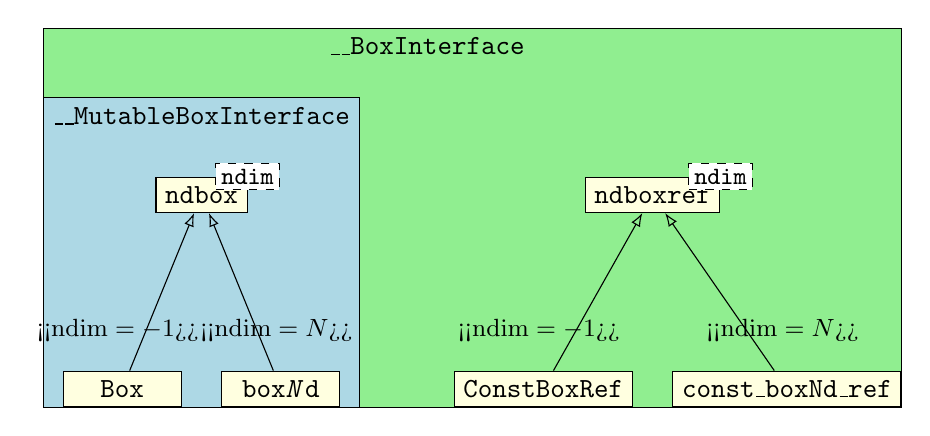
\begin{tikzpicture}[
  every node/.style={font=\tt},
  edge from parent path={[latex-] (\tikzparentnode.south) -- ++(0,-.5) -| (\tikzchildnode)}
  ]


  \node[align=center,below] (PI) at (0,0) {\_\_BoxInterface\\};
  \node[align=center] (MPI) [below left=0cm and 1.5 cm of PI, anchor=north] {\_\_MutableBoxInterface\\};


  \node[class, template={ndim}] (ndbox) [below left=1cm and 1.5 cm of PI, anchor=north] {ndbox};
  \node[class, template={ndim}] (ndboxref) [below right=1cm and 1.5 cm of PI, anchor=north] {ndboxref};

  \node[class, below left=2cm and 0.25cm of ndbox.south, minimum width=1.5cm] (Box){Box};
  \node[class, below right=2cm and 0.25cm of ndbox.south, minimum width=1.5cm]  (boxnd){box\emph{N}d};


  \draw[realization] (Box) -- (ndbox);
  \draw[realization] (boxnd) -- (ndbox);

  \node[above=0.25cm of Box, font=\small, align=center] { <<$\mathrm{ndim}=-1$>> };
  \node[above=0.25cm of boxnd, font=\small, align=center] { <<$\mathrm{ndim}=N$>> };


  \node[class,below left=2cm and 0.25cm of ndboxref.south] (BoxRef) {ConstBoxRef};
  \node[class,below right=2cm and 0.25cm of ndboxref.south] (boxndref) {const\_boxNd\_ref};
  \draw[realization](BoxRef) -- (ndboxref);
  \draw[realization](boxndref) -- (ndboxref);
  \node[above=0.25cm of BoxRef, font=\small, align=center] { <<$\mathrm{ndim}=-1$>> };
  \node[above=0.25cm of boxndref, font=\small, align=center] { <<$\mathrm{ndim}=N$>> };


  \begin{scope}[on background layer]
    \draw[fill=LightGreen] (MPI.west |- PI.north) rectangle (boxndref.south east);
    \draw[fill=LightBlue] (MPI.north west) rectangle (MPI.east |- boxnd.south);

  \end{scope}



  % \draw [latex-] (PI.340) -- ++(0,-.5) -| (CPR);



  \end{tikzpicture}
\end{document}